\chapter{Music learning applications in AR}

\section{Introduction}

The DVIC augmented mirror overlays various digital information on top of the natural reflection of the user's head and upper body. Such overlaid information can be useful for the learning of embodied skills, and applications have already been created for the mirror to help people learn sign language and dance.

Currently the most common way to learn singing is through: 
\begin{itemize}
    \item Recording and listening to one’s own performances. 
    \item Taking a good posture, which is important to learn to sing in tune.
    \item Paying attention to one’s breathing, which is the basis of vocal technique and can be improved through breathing exercises.
    \item Performing vocalization exercises, which require a lot of patience.
    \item A capella singing, practised by listening to and learning a piece many times before reinterpreting it. 
\end{itemize}
   

This project explores how the mirror can help people learn music, and in particular, singing. Seeing one's reflection is useful when practicing singing because it allows the monitoring of one's posture. The mirror adds the ability to monitor one's pitch accuracy. This is done by adding a frequency tracking module that estimates notes sung by the user and an interface that gives the user real-time visual feedback.
The user can then train his or her ability to sing in tune by comparing the target frequency with that actually sung. This ability is called musical imagery, the ability to "imaginate" a note before playing/singing it \cite{godoy2012musical}. It can be perfected with practice. This ability is very important for a musician as it allows him/her to visualise a gap between two notes he/she wants to play/sing, and to translate it on his/her instrument or by voice.

Practicing music can be very laborious, long, and difficult. For example, practicing singing requires attending singing classes that teach you to visualize the right note in your head before you sing it. Singing also requires good posture and breath control to be effective.
The interactive mirror has the potential to give users the ability to monitor their posture, an important element in singing. The user can get double feedback by singing in front of the augmented mirror. He can see the position of the notes in relation to the ones he is singing and can correct himself.
At the same time, he sees his reflection in the mirror and can correct his posture to sing more effectively. In order to implement the singing application, a frequency tracking module estimates the notes sung by the user, and the user interface gives feedback on the accuracy of his pitch.
The singer can also activate a tutorial with falling notes, activate the playback of music to learn it before singing it, and use a calibration to set the singable range of notes for him.

\section{Related work}

\subsection{Singing Learning Applications}

The development of new electronic musical interfaces gives rise to potential novel approaches in music education. The gestual interactive systems and interfaces have great potential for practice in music pedagogy \cite{farrugia2015tunes}.
A number of smartphone apps exist for people learning to sing that focus on giving feedback on correct intonation.
Yousician is a fairly comprehensive application that allows you to quickly learn and master piano, guitar, bass, singing, and other instruments by practicing on your real instrument.
It offers to learn music theory through special exercises and lessons. The application listens to the user singing/playing, evaluates his/her performance with a frequency estimation, and proposes to play different songs with tutorials and games. It offers a system of notes in the form of bars coming from the right, which the user must sing afterwards (see \ref{fig:yousician}). If he sings right, the bar turns green, if not, red.

\begin{marginfigure}
    \centering
    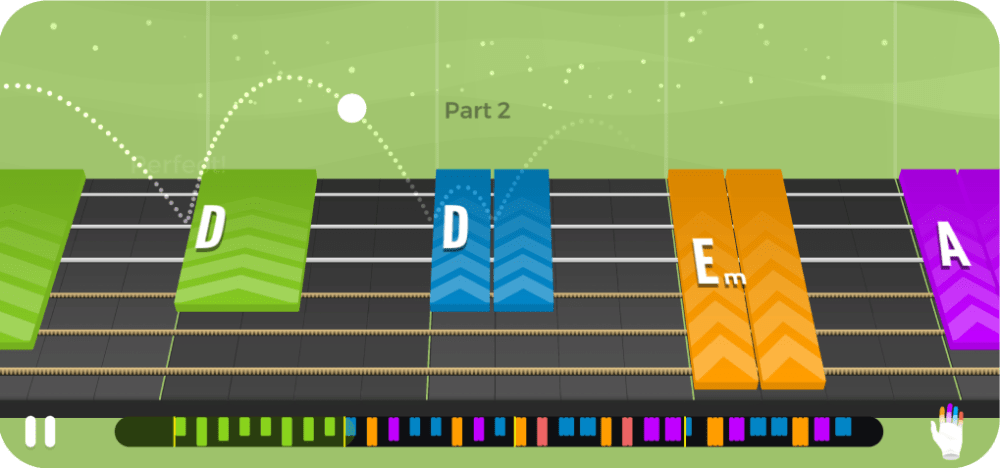
\includegraphics{AdrLfv_master_thesis/images/yousician.png}
    \caption{Yousician interface.}
    \label{fig:yousician}
\end{marginfigure}

Other applications are very similar such as Sing Sharp, LearnSing... Riyaz is another application that allows you to load existing music to generate the notes of the song, and then view a tutorial of these falling notes.
The application then gives statistics on the performance: pitch accuracy, control and breathing capacity, vocal range. These applications often start by determining a range of frequencies that the person can perform with the voice before starting the singing training. This allows the tutorial to be tailored to the user’s vocal abilities.

The general strategy of these applications is to use learning methods by practice, measurement, and correction. The classic operation is the realization of tutorials on the placement of the hands for an instrument, or the position of the notes to be sung for the note, then by a graphic feedback with the visualization of the fact that a note has been correctly sung or not.
It is possible to learn how to play music by means of video games created for this purpose. Among the best known video games in this field are Guitar Hero and Rock Band. These two games allow you to learn to play the guitar in a fun way, always using a system of falling notes \cite{farrugia2015tunes}.

\subsection{AR Music Practise}
Frederic Bevilacqua \& al. proposed a project with miniature wireless sensor system that is used with accelerometers and gyroscopes to make gesture recognition in musical pedagocial scenarios (see \ref{fig:Wireless-sensor-interface}). Music teaching methods are often based on playful approaches and exercises focusing on body movements. The project aimed to experience and practice “smoothness” and “fluidity” of musical gestures by analizing the curves of the movements \cite{bevilacqua2007wireless}.

\begin{marginfigure}
    \centering
    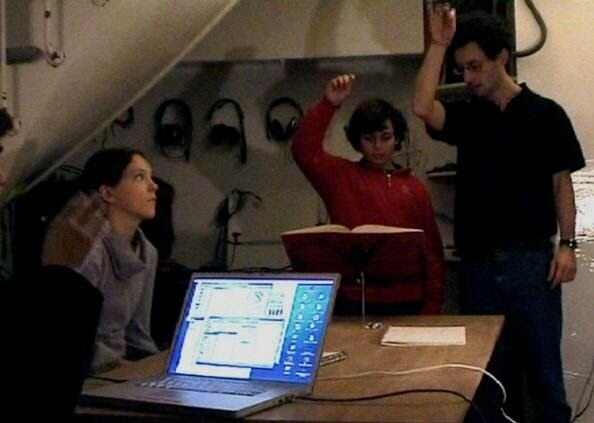
\includegraphics{AdrLfv_master_thesis/images/Wireless-sensor-interface.jpg}
    \caption{Teacher and student using the system during a music class \cite{bevilacqua2007wireless}.}
    \label{fig:Wireless-sensor-interface}
\end{marginfigure}

\begin{marginfigure}
    \centering
    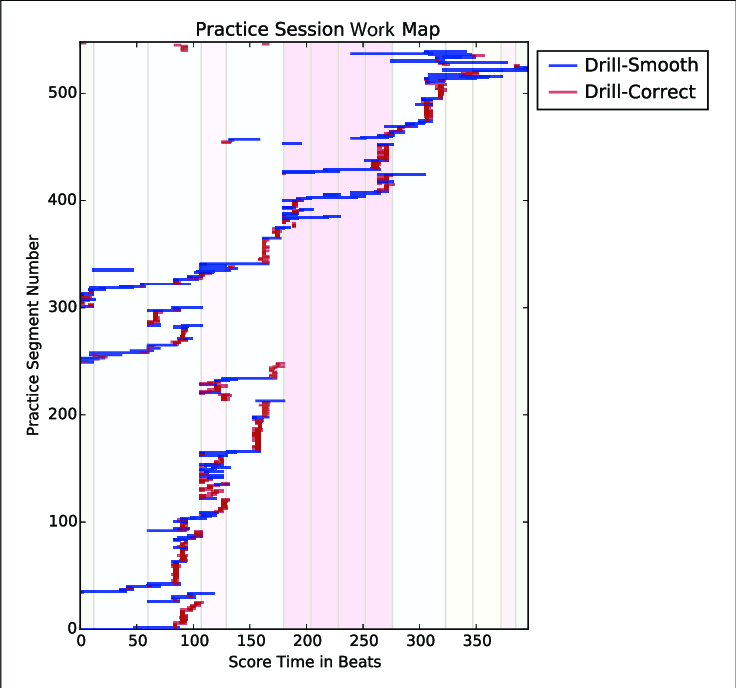
\includegraphics{AdrLfv_master_thesis/images/Practice-Session.png}
    \caption{Practice Session Work Map of an expert player (E-1)’s hour-long practice of Chopin’s “Mazurka in A minor, Op. 17 No. 4".}
    \label{fig:Practice-Session}
\end{marginfigure}

\begin{marginfigure}
    \centering
    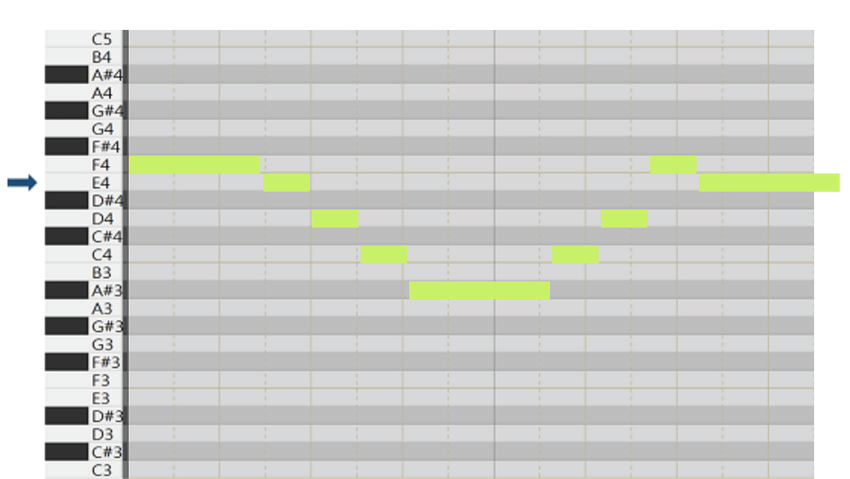
\includegraphics{AdrLfv_master_thesis/images/Intonation-Level-Classifier.png}
    \caption{Intonation Level Classifier with Song - Fly Me to the Moon \cite{lin2014implementation}.}
    \label{fig:Intonation-Level-Classifier}
\end{marginfigure}

Yu Ting Hang et al. proposed a visual interface for learning singing on the Internet. The aim is to link pitch and musical notation through frequency estimation and waveform recognition. The visualization of the sung notes in relation to the desired ones allows to correct vocal accuracy errors and thus to practice singing by sight \cite{huang2016visualized} (see \ref{fig:Practice-Session}).
Kin Wah Edward Lin et al. presented a self-learning tool for singing on the smartphone. It allows the user to improve timing and intonation in a similar way to the previous project. It uses an intonation level classifier, a user performance rating mechanism, and a pitch training tool. The mix of visual demonstration/feedback is natural to understand and useful (see \ref{fig:Intonation-Level-Classifier}). The user’s intonation score improved by an average of 94.81 \% after training.

\section{Singing Learning Program in AR}

\subsection{Context}

The DVIC augmented mirror project aims to change the way we perform certain tasks and disciplines in everyday life.
It adds a dimension of interactivity through our reflection, our position, our movements.

The mirror’s 3D camera makes it possible to precisely estimate the position of the user in  space. The person can then interact remotely, without touching the screen. A Plexiglas screen positioned above the screen of the device reflects the reflection of the user. This allows you to display elements over your reflection and thus interact with elements in augmented reality. The mirror’s augmentation gives people more awareness of their position and their movements. It allows full-body interactions with digital information, rather than accessing it through the small screens of computers and mobile devices. The added value of the project is to exploit mainly kinesthesia (which is not possible with other more traditional devices) as well as other forms of interaction. This is in addition to the various ways of interacting with the human body (human inputs/outputs) that can be exploited by the electronic devices we use every day.

Applications allow for example to have a return of its position with the display of a mediapipe skeleton above its reflection, to learn elements of sign language thanks to a training module, as well as to test other games. One of the primary uses of the mirror is to enable much better learning, using as many forms of intelligence as possible.

\subsection{Overview}

The objective of the project is to be an example of a module allowing people to learn the practice of a musical instrument on the mirror. As the device only requires the person in front of it without any material, a musical module would not have been suitable for most musical instruments.
The project is based on frequency estimation for practice. A user plays an instrument or sings in front of the mirror (see \ref{fig:xiao_singing}). The mirror collects the frequency emitted and displays it on the screen.

\\TODO Refaire cette photo

\begin{figure}[h]
    \centering
    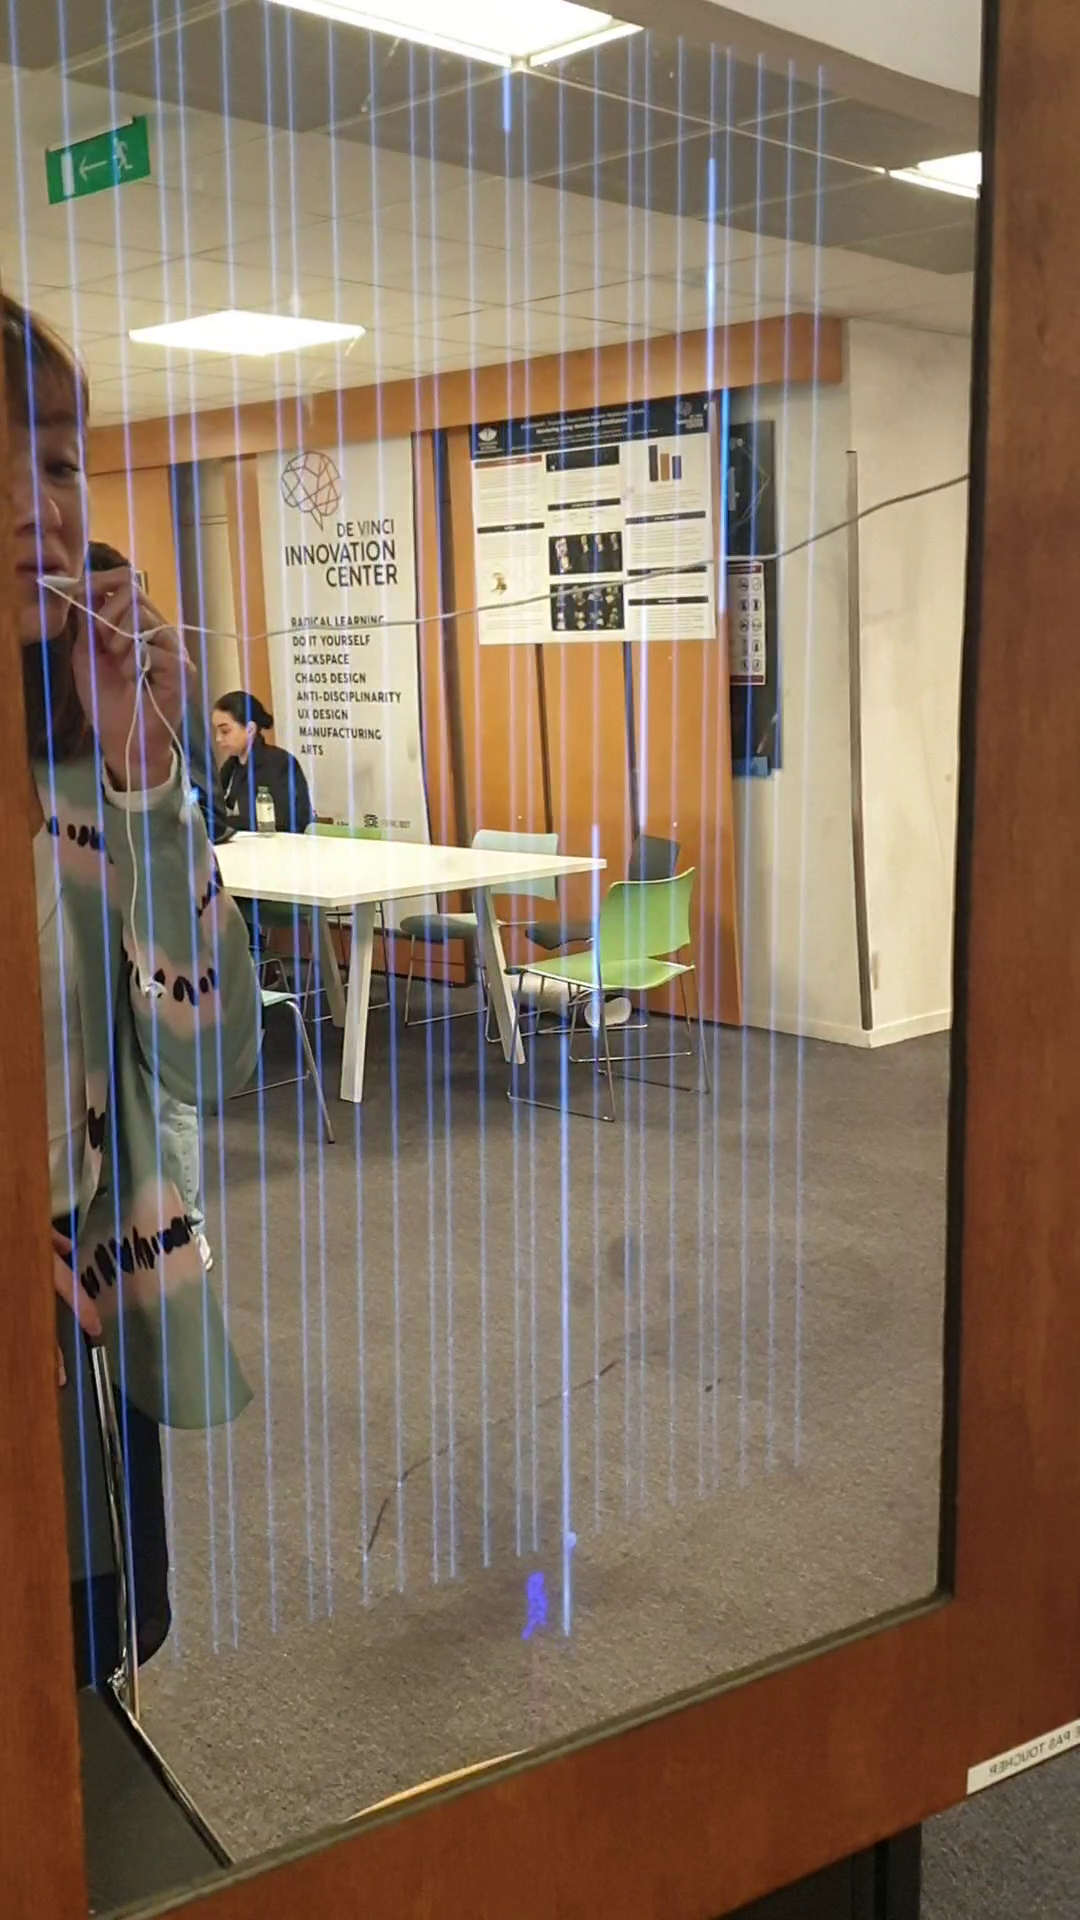
\includegraphics[width=2.2\columnwidth]{AdrLfv_master_thesis/images/xiao_singing.png}
    \caption{A use case of the musical training application on the augmented mirror.}
    \label{fig:xiao_singing}
\end{figure}

The user sees the frequency he or she is emitting represented by a dot on the screen with a particle effect. The lower the frequency, the further to the left the dot is, and vice versa. Some options can be launched from the sub-menu of the "music\_training" application already
implemented on the mirror. The user can launch different music tutorials.

For example, he can launch the tutorial "La vie en rose", notes fall from the top of the screen and he must play them in rhythm. The module no longer has any aspect related to movement or position but only to the frequency emitted by the instrument or by the voice.
When the user sings correctly, the bars falling from the top change colour, gradually turning green and the particle effect on the dot intensifies (see \ref{fig:music_training}). They become increasingly red when the user sings out of tune. The score achieved is displayed for a few seconds at the end of the song.

\begin{figure}[h]
    \centering
    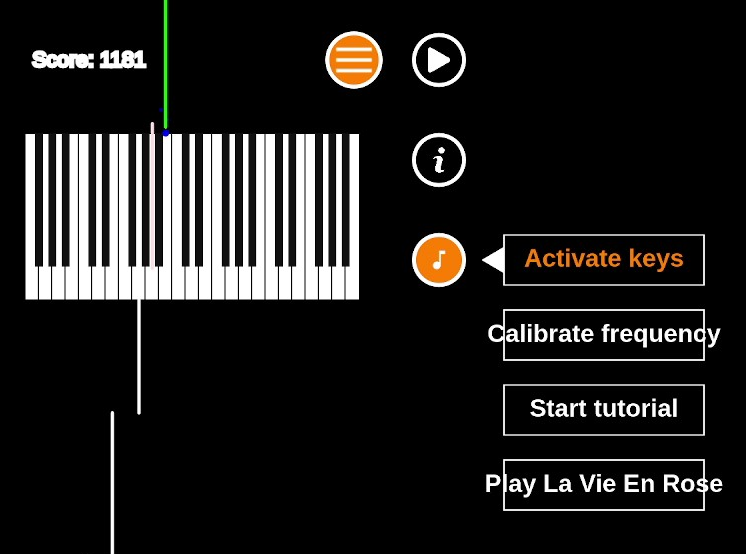
\includegraphics[width=2.2\columnwidth]{AdrLfv_master_thesis/images/music_training.png}
    \caption{The interface of the music learning application.}
    \label{fig:music_training}
\end{figure}

The vision of the project is to train the user to more or less consciously link the manipulation of the instrument or his voice with the sound he visualises in his head. The visual present on the mirror allows him to know where he is, if he has played/sung the right note and how to correct it if not.
This approach is different because it offers different options in the display. The user can launch different music tutorials, display bars to locate notes, erase them, as well as display the position of his hands.
Practising on a mirror is a plus as the user practices standing up unlike with a telephone. This makes it easier to practice singing because the body remains upright. This project is intended to be suitable for multiple instruments, while being entertaining and instructive.

\subsection{General Architecture}

The augmented mirror system runs on an operating system software called GOSAI. The music practice module takes the form of a JavaScript application coded directly on it. It uses the P5 library to display 2D elements and create the sketch. The backend will use two drivers coded on GOSAI for the occasion: a new driver allowing GOSAI to use the microphone of the device used and a driver allowing to make frequency estimation listening to the microphone. The latter takes a sound wave generated at the input and returns a musical frequency.

The GOSAI microphone driver takes the audio stream from the device hardware. It passes the data to the "frequency\_estimation" module which detects the frequency emitted in the audio stream as well as the gain and other parameters. This module places this data in the Reddis data. The processing.py file retrieves the frequency estimation data from the data and sends it to the display.js with socket.io. The display initializes a new music workout and sends it the necessary data to run.

New various tools such as the sub-menu system are coded on GOSAI for the project. The sub-menu allows GOSAI applications to propose options to be activated or deactivated manually by the user thanks to the estimation pose according to his desires.

\subsection{Posture Adjustment}



\section{Theremine Learning Program in AR}

\subsection{Overview}


\subsection{General Architecture}


\subsection{Position Correction Visualisation}



\section{Correction in AR}


% \section{Tests}

% \subsection{Quantitative Tests}

% The application must be responsive for perfect practice. The delay measured between the note being sung and its display on the mirror should be as small as possible. It can be measured by placing timers between the detection of a new note in the microphone driver in the backend, and then at the output when the note is displayed in the JS application in the frontend.
% The measured pitch must also be accurate enough to allow a qualitative estimation of the sung note. The Hertz value measured by the frequency estimation must be accurate enough to make a difference between two notes.

% \subsection{User Tests}

% The user tests in this project aim to assess a user’s facilitation of learning to sing with the
% mirror compared to other conventional tools.

% \paragraph{Evaluation of the user learning}

% The difference between classical learning through "a capella" practice and learning with dynamic correction on the mirror is evaluated. A randomly chosen user is given 10 seconds of the song "Edith Piaf - La foule" played on the piano [6] (from 0:20). Then he is asked to sing 10 seconds of the "singing" part again. We record the estimated notes during his singing thanks to a frequency estimation application. Then we make him use the
% application on the mirror teaching him 10 seconds of the song "La vie en rose" from Edith Piaf (using the built-in music player). Using the same frequency estimation application on the smartphone, we record an estimate of the notes that the user sings. These data are then compared to study the best performance.

% \paragraph{Evaluation of the user experience}
% Here are the areas evaluated and the questions asked to the tested users. Their opinion is measured with a score out of 10 points.
% Evaluation of the motivation to learn with this type of interaction: -Average motivation to learn this particular way. -Average fun in interacting.
% Evaluation of the comprehensibility of the module: -Ease of understanding what needs to be done Evaluation of the estimation/display system: -Usability of the overall system, responsiveness, accuracy, smoothness of display. -Practicality of the design, position of the notes, graphics chosen for the different elements. The rendering estimated and displayed in the application should be smooth and not display any other spurious frequencies measured by the microphone. Problems of this kind can lead to the display of unsung frequencies as well as "skipping" of the cursor displaying the sung note. 

% Evaluation of the tutorial method with falling notes. -Relevance and effectiveness of the tutorial method with falling notes rather than another.
% Evaluation of the use of the reflection. -Does the use of the reflection in the glass seem to be a good potential for improving one’s vocal practice. Finally, the subject is asked about their remarks, suggestions and other constructive comments about the project.

\section{Conclusion}
